\documentclass[a4paper, twoside, openright]{report}
%\usepackage[utf8x]{inputenc}
\usepackage[a4paper,top=2cm,bottom=2cm,left=2cm,right=2cm,marginparwidth=2cm]{geometry}
\usepackage[T1]{fontenc}
\usepackage{lmodern}
\edef\restoreparindent{\parindent=\the\parindent\relax}
\usepackage[parfill]{parskip}
\restoreparindent
\usepackage{tocloft}
\usepackage{afterpage}
% \usepackage[french]{babel}
\usepackage[babel=true,kerning=true]{microtype}
\usepackage[acronym]{glossaries}
\usepackage{amssymb}
\usepackage{amsmath}
\usepackage{hyperref}
\usepackage{phonenumbers}
% \usepackage{fancyhdr}
% \pagestyle{fancy}
\usepackage[backend=biber]{biblatex}
\addbibresource{src/bibliography.bib}
\usepackage{appendix}
\usepackage{float}
\usepackage{graphicx}
\usepackage{subfig}
\usepackage{svg}
\usepackage{multirow}
\usepackage[table,xcdraw]{xcolor}
\usepackage{colortbl}
\usepackage{tikz}
\usepackage{minted}
\usepackage{color}
\usepackage{xcolor}
\usepackage{csquotes}
\usepackage{rotating}

\setlength{\cftbeforelottitleskip}{1em}
\setlength{\cftbeforeloftitleskip}{1em}
\setlength{\cftbeforetoctitleskip}{1em}

\setlength{\cftafterlottitleskip}{1.5em}
\setlength{\cftafterloftitleskip}{1.5em}
\setlength{\cftaftertoctitleskip}{1.5em}

\newcommand{\figwidth}{15cm}

\newcommand\blankpage{
    \null
    \thispagestyle{empty}
    \addtocounter{page}{-2}
    \newpage}

\newcommand\emptypage{
    \null
    \newpage}

% Command to create a glossary entry with correspondent acronym.
% https://tex.stackexchange.com/questions/8946/how-to-combine-acronym-and-glossary
% Args : 1: entry, 2: acronym/name, 3: long name, 4: description
\newcommand{\newglossaryentrywithacronym}[4]{
    %%% The glossary entry the acronym links to   
    \newglossaryentry{#1_gls}{
        name={#2},
        long={#3},
        description={#4}
    }

    % Acronym pointing to glossary
    \newglossaryentry{#1}{
        type=\acronymtype,
        name={#2},
        description={#3},
        see=[Glossary:]{#1_gls}
    }
}

\definecolor{LightGray}{gray}{0.9}

\newminted[pythonCode]{python}{
    frame=lines,
    framesep=2mm,
    baselinestretch=1.2,
    bgcolor=LightGray,
    fontsize=\footnotesize,
    linenos}

\newminted[outputCode]{bash}{
    frame=lines,
    framesep=2mm,
    baselinestretch=1.2,
    bgcolor=LightGray,
    fontsize=\footnotesize,
    linenos}

% \setlength{\headheight}{28pt}
% \fancyhead[L]{ALLEMAND Fabien}
% \fancyhead[C]{}
% \fancyhead[R]{\includegraphics[scale=0.025]{/home/fabien/logo_TSP_1.jpg}}
% \fancyfoot[L]{}
% \fancyfoot[R]{}

\makeglossaries

\newacronym{lic}{LIC}{Learned Image Compression}
\newacronym{clic}{CLIC}{Challenge on Learned Image Compression}
\newacronym{psnr}{PSNR}{Peak Signal to Noise Ratio}

% \newglossaryentry{front_end}
% {
%         name={front end},
%         description={}
% }


\begin{document}

\thispagestyle{empty}
\begin{center}

\vspace*{2.5cm}

{\fontsize{30}{30}\selectfont PRIM Project}

\rule{\textwidth}{1pt}

\medskip

{\fontsize{22}{22}\selectfont Learned Image Compression on FPGA}

{\fontsize{18}{18}\selectfont Intermediate Report}

\rule{\textwidth}{1pt}

\medskip

{\fontsize{18}{18}\selectfont Supervisors: Attilio Fiandrotti, Alaa Mazouz, Sumanta Chaudhuri}

\medskip

{\fontsize{18}{18}\selectfont Student: Fabien ALLEMAND}

\medskip

{\fontsize{14}{14}\selectfont 2024 - 2025}

\vspace*{2.5cm}

\includegraphics[height=4cm]{/home/fabien/logo_TSP_3.png}

\vfill

\end{center}

\afterpage{\blankpage}

\newpage
\pagenumbering{roman}

% \input{src/contact.tex}

\chapter*{Acknowledgments}
Working on a six-month research project at the Institut Polytechnique de Paris has been an enriching experience, marked by numerous technical discoveries. I would like to express my gratitude to everyone who has supported and guided me throughout the project and in the writing of this report.

First and foremost, I would like to thank my supervisors, Attilio Fiandrotti, Alaa Mazouz, and Sumanta Chaudhuri, researchers at the Institut Polytechnique de Paris, for their warm welcome, the valuable time spent together, and the knowledge they shared with me.

I would also like to extend my sincere thanks to Alaa Mazouz, who directly supervised my work and collaborated with me throughout the project. His ongoing support and detailed explanations were crucial in helping me understand the tasks entrusted to me and in acquiring new skills that will undoubtedly benefit my future endeavors.

\printglossary[type=\acronymtype]
\printglossary

\newpage
\listoftables

% \afterpage{\emptypage}

\newpage
\listoffigures

\afterpage{\emptypage}

\newpage
\tableofcontents

\afterpage{\emptypage}

\newpage
\pagenumbering{arabic}

\chapter*{Introduction}
\addcontentsline{toc}{chapter}{Introduction}
Since the beginning of computers, the amount of raw data has always exceeded the capacity of storage mediums. With the quantity of created data approaching 500 terabytes every day in 2024, data compression has become ubiquitous. Whether it is to improve storage capacity or enhance data transfer, data compression is used regardless of the scale. Let us focus on image data. Image files on a computer disk can be compressed to take less storage space. Video streams of data transfered over the internet are compressed in order to make transfers more efficient in terms of resource availability and energy consumption. Both examples highlight the induced improved user experience (ability to store more files on the same disk and fast download speeds).

However data compression comes at a cost. There is a limit to how many bits can be removed while encoding the exact same data. Past this limit, some data is lost which can degrade the content of the file to various degrees. This process, called lossy image compression (as opposed to lossless compression), introduces a tradeoff between data compression and data quality. There is a wide variety of (deterministic) algorithms used to compress data. Some of them are designed to focus on compression at the cost of quality. Such algorithms (like GIF) work well for simple schematics and diagrams but introduce artifacts on more complex files like photographs. State of the art algorithms (like JPEG or Webp) manage to perform data compression while preserving the majority of the file content. Some artifacts can be added but they can be negligeables depending of the use case (for instance they are often not visible to the human eye without close inspection).

With the recent progress of machine learning, new compression algorithms appeared. These probabilistic algorithms are based on neural networks that can learn a better way to encode data with a minimum number of bits. The only issue being that these methods require way more processing power than previous state of the art compression algorithms. The goal of this project is to achieve real-time image compression on resource constrained platforms. Chapter \ref{sota} summarises state of the art methods. The first results achieved in the context of this project mainly consist in reproducing state of the art results and are presented in Chapter \ref{results}.
% Section \ref{lic} explains how machine learned image compression works and Section \ref{sota} briefly presents state of the art methods. Finally, ... of this project is shown in Section \ref{results}.

\chapter{Learned Image Compression}
\label{lic}

\chapter{State of the Art}
\label{sota}
\acrfull{lic} is a lossy compression method based on machine learning. Using autoencoder architecture, it is possible to build and train end-to-end a neural network that achieves balance between image compression efficiency and reconstruction fidelity. \acrshort{lic} consists of three successive steps: projection in a low-dimensional latent space (using the encoder part of the autoencoder), quantisation and lossless entropy coding. Decompression is achieved by applying entropy decoding and projecting the result back into the image space with the decoder part of the autoencoder \cite{licmedium, licstanford}.

Early seminal works accounted for a unique latent representation modelled with a fully factored distribution \cite{ballé2017endtoendoptimizedimagecompression}. Since then, much of the research in the field has focused on improving the compression efficiency by refining the entropy model. This basic scheme was then improved by introducing an auxiliary latent space called hyperprior capturing spatial correlation within the image, furthering compression efficiency \cite{ballé2018variationalimagecompressionscale}. \acrshort{lic} has shown the ability to outperform standardised video codecs in compression efficiency, fostering the demand for embedded hardware implementations.

Applying frugal machine learning techniques can help reducing the load of the neural network on the computer. Such methods include pruning, quantisation or knowledge distillation \cite{touvron2021trainingdataefficientimagetransformers}. It should be noted that knowledge distillation can be achieved between different architecture opening the possibility to use a completely different network for decoding \cite{liu2022crossarchitectureknowledgedistillation}.

Achieving real-time coding on resource constrained platforms such as FPGAs demands ad-hoc design choices such as in the state of the art \acrshort{lic} implementations. However, FPGA implementations have been lagging behind recent research in \acrshort{lic} due to the increasing complexity of implementing in hardware recent \acrshort{lic} models. For example, further improves the RD efficiency by introducing slice-based latent channel conditioning and latent residual prediction with an approach suitable for parallel execution. The RD efficiency is further boosted in the work of Zou et al. \cite{zou2022devildetailswindowbasedattention} by introducing a Window Attention Module in the autoencoder architecture and experimenting with a transformer-based architecture in place of the traditional convolutional architecture.

\chapter{Reproducing Results}
\label{part_1}
This chapter is dedicated to our ability to achieve results similar to state-of-the-art models as well as our method to evaluate them. In the first section, we introduce the tools we use to achieve results similar to these reference models. Our methodology and results are described in the second section.

\section{Tools}
As explained in chapter \ref{sota}, current \acrshort{lic} models achieve impressive results: they provide encoding of images that contain very few bits while preserving their content. However, these models require a lot of processing power making them unsuitable for realtime application on resource constrained devices. The goal of this project is to explore solutions to reduce the processing power used by these models, potentially leading to realtime image compression/decompression on such devices. In order to do that, it is necessary to have access to the state-of-the-art \acrshort{lic} models, the image datasets used to train them and enough processing power to train such models.

CompressAI \cite{compressai} is a Python library for learned compression. Based on the well known machine learning library PyTorch, compressAI provides custom operations, layers and models for deep learning based data compression and pre-trained end-to-end compression models for \acrshort{lic}. Amongs the pre-trained models is the model from Ballé et al. \cite{ballé2018variationalimagecompressionscale} that will be used throughout the project.

Usually, researchers train their models on the OpenImages dataset \cite{openimages} but pre-trained models on compressAI have been trained on the Vimeo90K dataset \cite{xue2019video}. In order to perform proper model comparisons, the Vimeo dataset will be used for training in this project. For testing, two datasets will be used: the Kodak dataset \cite{kodak} and the dataset from the \acrfull{clic} \cite{clic}. Similarly to compressAI, visual inspection are also performed on a photograph of the port of Saint-Malo available in the GitHub repository of the library.

The computing power required for training and using models will be provided by the GPU cluster of Télécom Paris.

\section{Results Reproduction}
In a research project, reproducing state-of-the-art results is key. The first thing to do is to ensure that our work environnement is correct by reproducing results from articles. This also provides shared baseline results between papers and our work, that is used to compare our future results.

For this project, we selected the scale hyperprior model introduced in 2018 by Ballé et al. \cite{ballé2018variationalimagecompressionscale}. This model has the advantage of being straightforward and yet complex enough to be challenging but not impossible to run on ressource constrained computers. Its simple two stages architecture (described in \ref{}) makes it a suitable candidate to perform knowledge distillation experiments including using the latent spaces. As experiments parameters are not disclosed in the paper, we try to reproduce results from the compressAI library, that is to say: achieve the same results as the pre-trained model from the model zoo.

The training methodology used by compressAI is described in the documentation \cite{compressai_train}. Models were trained between 4 and 5 million steps on 256x256 image patches randomly extracted and cropped from the Vimeo90K dataset. The batch size is 16 or 32 (we choose 16). The initial learning rate is 1e-4 and decreases over time (it is divided by 2 when the evaluation loss reaches a plateau). Two different metrics can be used: MSE or MS-SSIM. We keep the default metric (MSE) which corresponds to using the following loss function: \(L = \lambda * 255^{2} * D + R\) with \(D\) and \(R\) respectively the mean distortion and the mean estimated bit-rate. The parameter \(\lambda\) allows to adjust the tradeoff between compression and image quality. Higher values give more importance to distortion encouraging the model to produce reconstructed images with high quality at the expense of bit-rate. Inversely, lower values of \(\lambda\) imply more compression and more data loss. CompressAI proposes 8 pre-trained models with different values of \(\lambda\) represented by the argument \textsf{quality}. The correspondance between this argument and the value of \(\lambda\) is summarised in Table \ref{tab}. It is important to note that the \textsf{quality} argument in compressAI also impacts the network architecture (number of channels and size of the latent space).

\begin{table}[]
    \centering
    \begin{tabular}{|l|c|c|c|c|c|c|c|c|}
    \hline
    \textsf{quality}                      & 1 & 2 & 3 & 4 & 5 & 6 & 7 & 8 \\ \hline
    Value of \(\lambda\) for MSE & 0.0018 & 0.0035 & 0.0067 & 0.0130 & 0.0250 & 0.0483 & 0.0932 & 0.1800 \\ \hline
    \end{tabular}
    \caption{Correspondance between the argument \textsf{quality} in compressAI and the value of \(\lambda\) when using MSE}
    \label{tab}
\end{table}

This part of the project is divided in two parts. First, we try to train a single model and compare it to other pre-trained models. Then we train several models in order to produce rate-distortion curves.

\subsection{Single Model}
Using the training script provided by compressAI and following the methodology, we train a scale hyperprior model with the compressAI argument \textsf{quality} set to 3, which corresponds to an architecture with 128 channels and 192 channels in the expansion layers (i.e. size of the image latent space). The model is trained for approximately one million steps.

% UPDATE RESULTS
After training the model is evaluated and compared to pre-trained models. First, we try a single inference with this newly trained model. Figure \ref{balle_repro_1} shows that the reconstructed image (middle) is visually close to the original image. However, the difference between the two images (right) reveals that there are a lot of differences. These differences are located in the part of the image that contains details. These parts are often refered as containing high frequencies and are particularly hard to compress as opposed to low frequency areas (like the sky in this picture) that do not contain a lot of information. In this specific example, we found these differences are mainly noticeable in the clouds and the water that appear smoother on the reconstruction.

\begin{figure}
    \centering
    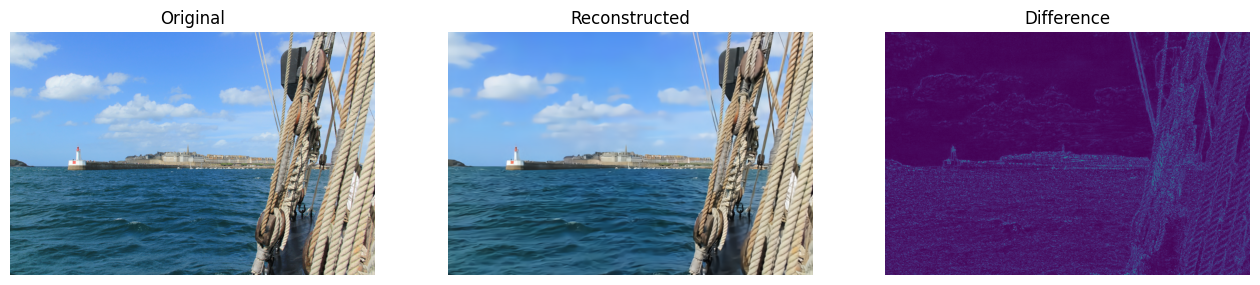
\includegraphics[width=15cm]{img/balle_repro_1.png}
    \caption{Comparison of the reconstructed image with the original image. At first glance, the reconstructed image (middle) looks very similar to the original (left). Further inspection using the difference between the two images (right) unveils the loss of details attributed to lossy image compression/decompression. As expected, parts of the image containing details are the most affected whereas plain areas are untouched.}
    \label{balle_repro_1}
\end{figure}

Figure \ref{balle_repro_2} shows encoding of the image at the same bit-rate using different methods. It is clear that the network (top right) is the more accurate among the three methods used: the reconstructed image is closer to the original image. JPEG introduces a lot of artifacts (blocs) and Webp does not retains as much details as the network, especially in the water.

\begin{figure}
    \centering
    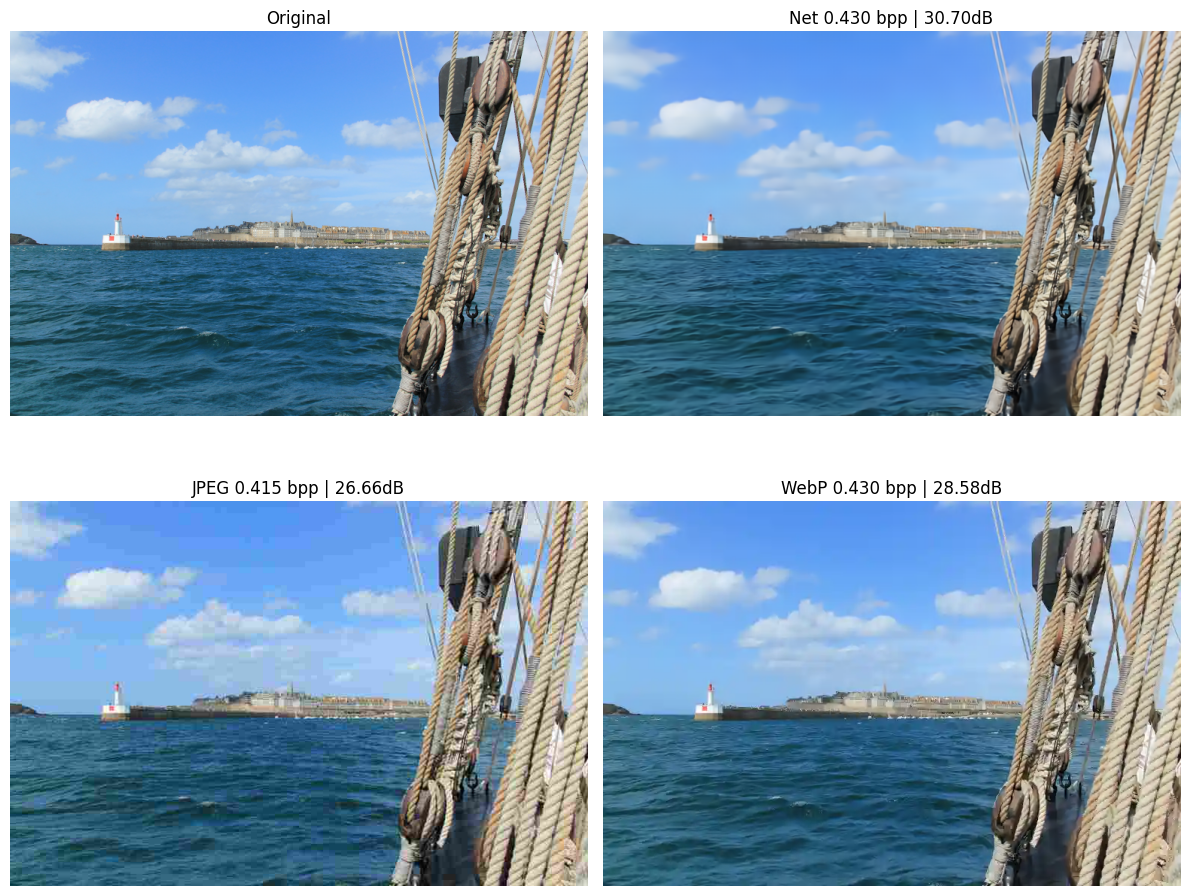
\includegraphics[width=15cm]{img/balle_repro_2.png}
    \caption{Comparison to classical codecs: quality coparison at similar bit-rate}
    \label{balle_repro_2}
\end{figure}

For the same distortion rate, our model manages has the smallest bit-rate out of the three methods, that is to say: for the same visual quality, measured by the \acrful{psnr}, the image is more compressed. Figure \ref{balle_repro_3} shows that it achieves less than 0.5 bits per pixel whereas traditional compression methods like Webp or JPEG achieve respectively 0.698 and 1.054 bit per pixels.

\begin{figure}
    \centering
    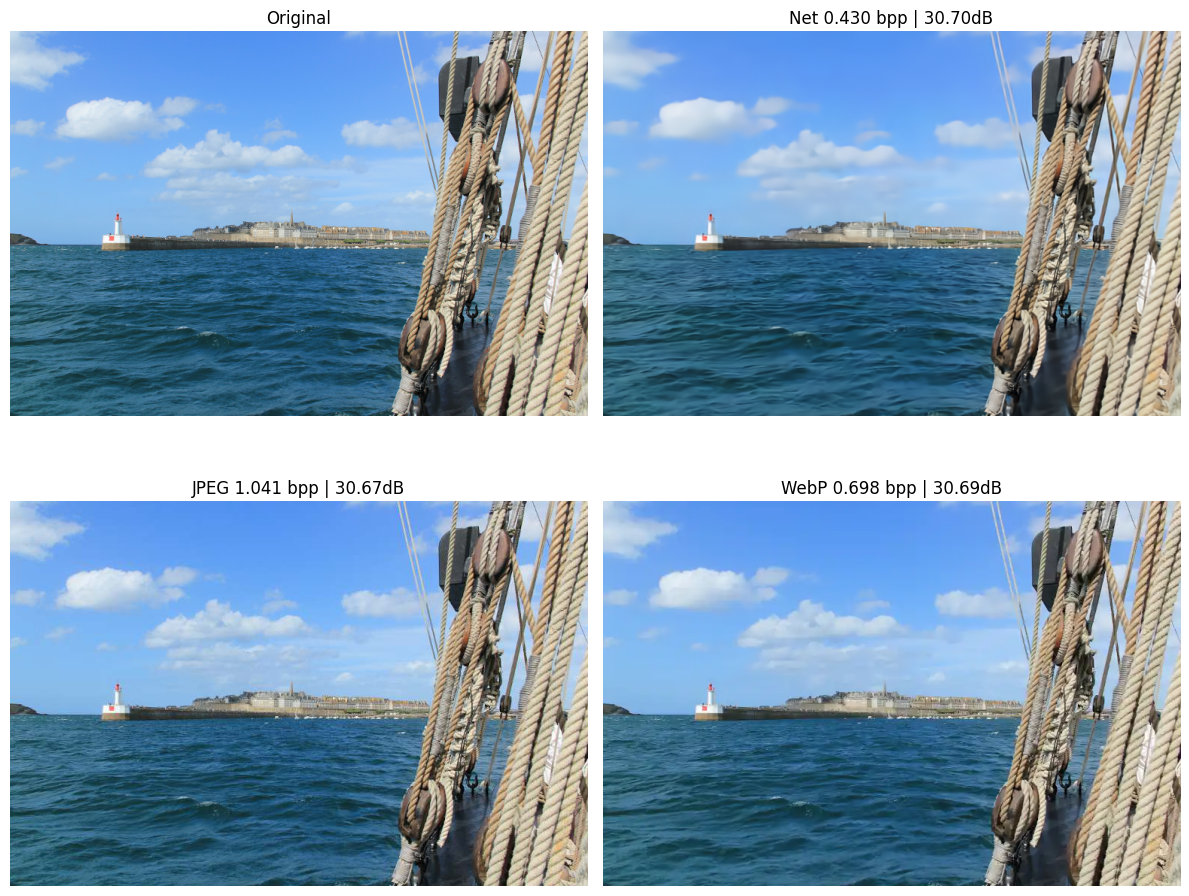
\includegraphics[width=15cm]{img/balle_repro_3.png}
    \caption{Comparison to classical codecs: bit-rate coparison at similar PSNR}
    \label{balle_repro_3}
\end{figure}

Similar results are observed on Figure \ref{balle_repro_4} which is based on MS-SSIM, another method to measure visual fidelity.

\begin{figure}
    \centering
    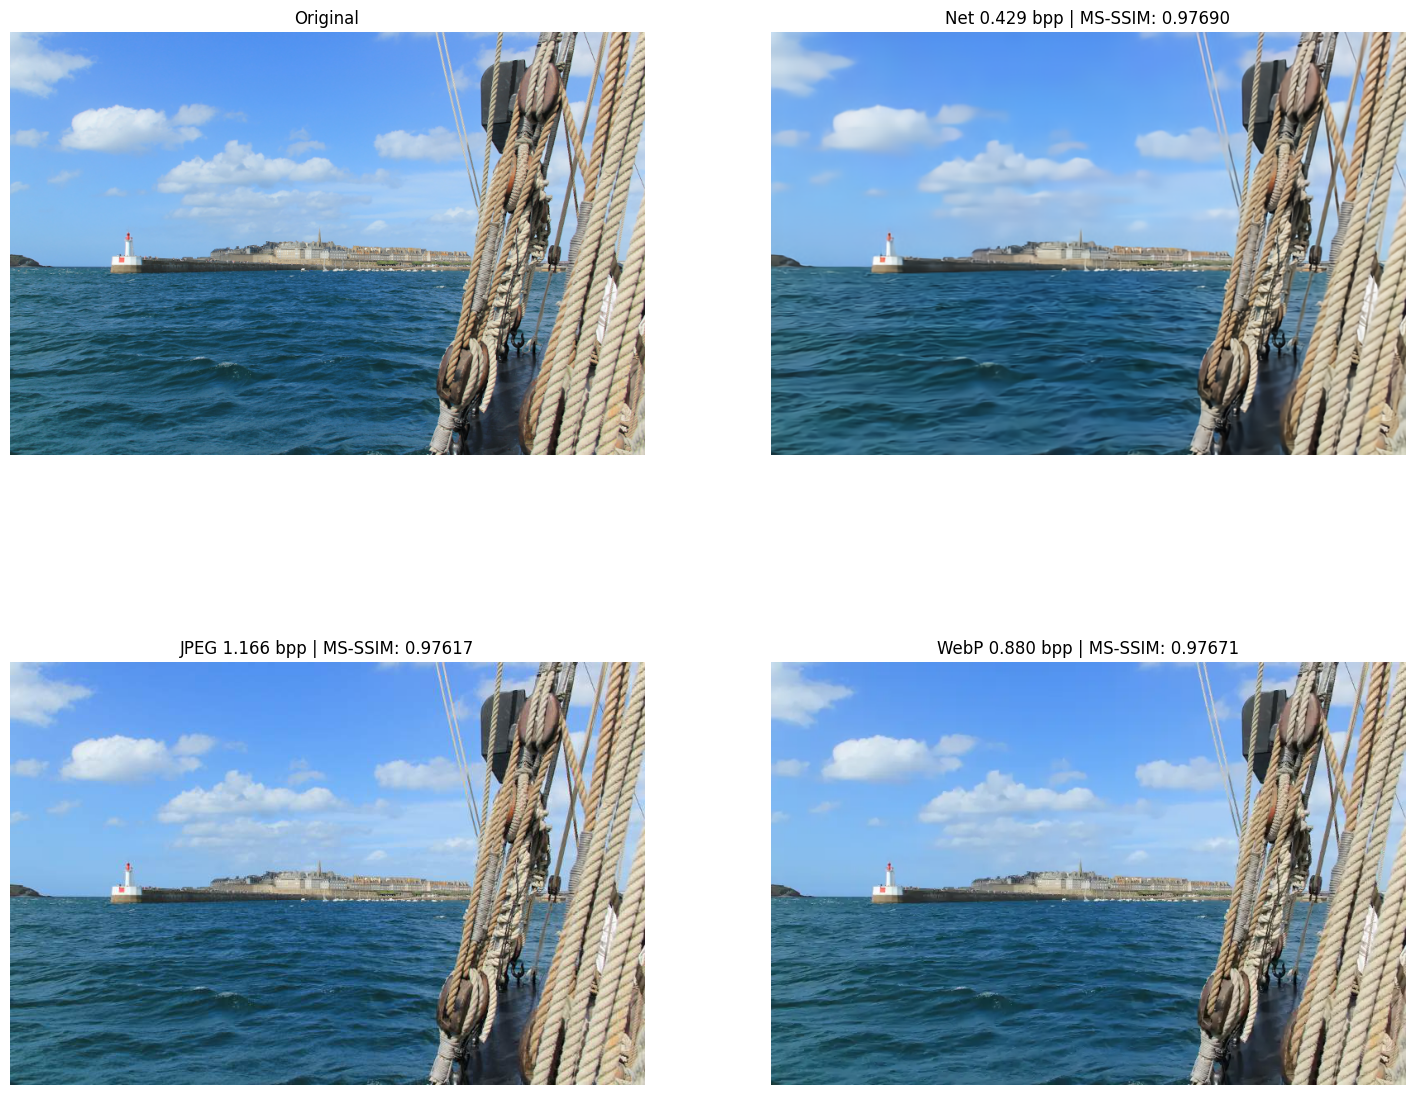
\includegraphics[width=15cm]{img/balle_repro_4.png}
    \caption{Comparison to classical codecs: bit-rate coparison at similar MS-SSIM}
    \label{balle_repro_4}
\end{figure}

Finally, we compare our models to other \acrshort{lic} models accessbible in the compressAI model zoo. Figure \ref{balle_repro_5} allows to compare visual results from our model at three stages of the training and various pre-trained models. Results are visually close but, by zooming, it is clear that our models retain more details than the other pre-trained models (for intance in the ropes). This is coherent with Figure \ref{balle_repro_6} that shows that our models are more focused on quality at the expense of bit-rate (located in the top right of the plot). Other models perform worse in term of image quality but achieve a lower compression rate (bottom left of the plot).

\begin{figure}
    \centering
    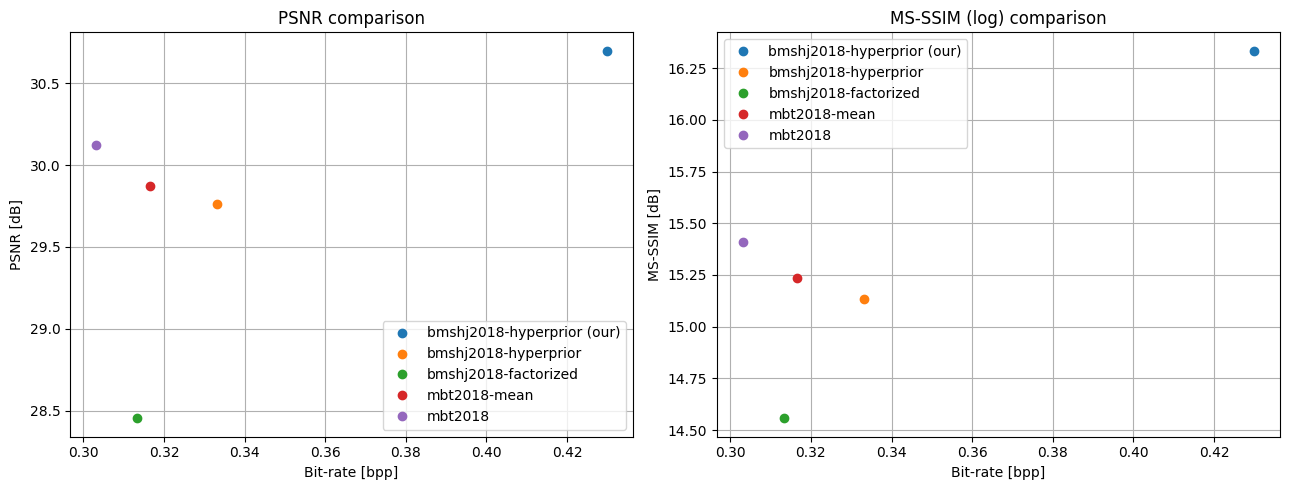
\includegraphics[width=15cm]{img/balle_repro_5.png}
    \caption{Comparison to other \acrshort{lic} models: image reconstruction}
    \label{balle_repro_5}
\end{figure}

\begin{figure}
    \centering
    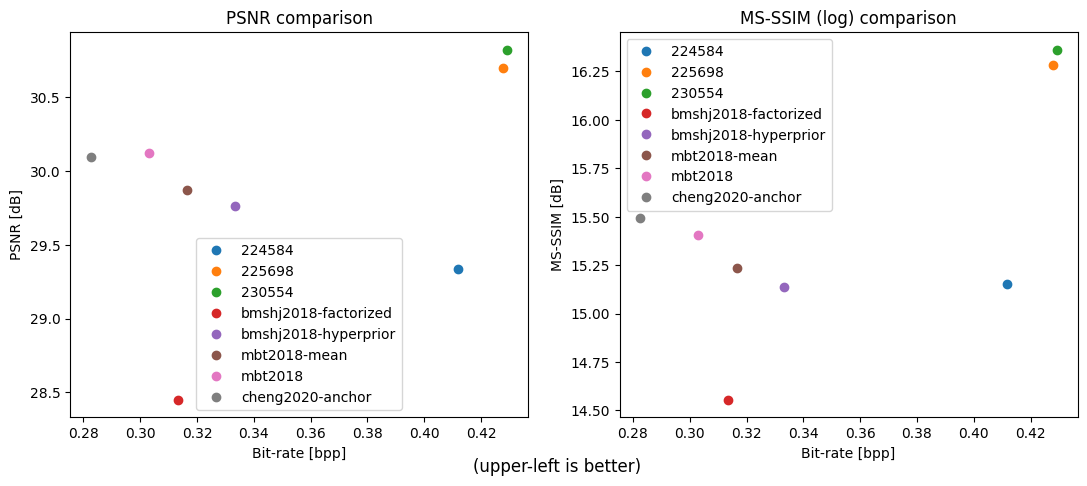
\includegraphics[width=15cm]{img/balle_repro_6.png}
    \caption{Comparison to other \acrshort{lic} models: rate-distortion curves}
    \label{balle_repro_6}
\end{figure}

This section show that we are able to train a \acrshort{lic} model able to compress and reconstruct images while mostly preserving its content. Our model performs better than deterministic codecs like JPEG or Webp but does not produce the same results as the pre-trained ones. It should be noted that, at this point, we are mainly checking if training is working properly on the GPU cluster and that we are now comparing models that were trained differently. Next section focuses more on the models parameters and the impact on the bit-rate/distortion tradeoff.
% END UPDATE RESULTS

\subsection{Rate-Distortion Curves}
% Different applications require different tradeoffs in terms of bit-rate and image quality. While bandwith limited video calls require low bit-rate at the expense of image quality, transferring a single high resolution artistic picture necessitates is more focused on image quality than preserving bandwidth.
Rate-distortion curves are a common tool to compare \acrshirt{nn} architectures in \acrshort{lic}. It consists in plotting the average distortion in function of the average bit-rate evaluated on a set of images. Using a range of rate-distortion tradeoffs allows to easily evaluate and compare the overall \acrshort{rd} performance of an architecture.

Using the training script provided by compressAI and following the methodology, we train 8 different models: one for each value of the compressAI \textsf{quality} argument. That is to say, one for each couple of value of \(\lambda\) and corresponding model architecture. However, to quickly achieve comparable results, we limit the number of epochs to 65, just under what the GPU cluster is able to compute in 24 hours.

Let us start by passing a single image through the networks. The image from the Kodak datset is compressed and decompressed before being cropped for easier comparison. Figure \ref{bdpsnr_1} shows image reconstruction results from our models and pre-trained models for each settings. Models with the same \acrshort{rd} tradeoff from the compressAI zoo or trained from scratch produce results that are visually very similar. As expected, there is a discernable shift in image quality accross the range of models. Images related to lower values of \(\lambda\) (low bit-rate and low quality) lack details and appear blurry. At the other end of the spectrum, images correponding to higher values of \(\lambda\) (high bit-rate and high quality) look more detailed, sharp and similar to the original image. Notice how the details in the faces and the water appear when the value of \(\lambda\) increases.

\begin{figure}[H]
    \centering
    \subfloat[Our networks]{{\includegraphics[width=8.5cm]{/home/fabien/TSP/3A/PRIM/bdpsnr/test_res/20241129_085637/networks_kodak_kodim14.png} \label{bdpsnr_1:a}}}
    \subfloat[Pre-trained networks]{{\includegraphics[width=8.5cm]{/home/fabien/TSP/3A/PRIM/bdpsnr/test_res/20241129_085637/pretrained_networks_kodak_kodim14.png} \label{bdpsnr_1:b}}}
    \caption{Reconstruction results on image 14 of the Kodak dataset. For a given \acrshort{RD} tradeoff, our models produce results visually similar to the pre-trained models. The level of ddetail increses with the value of \(\lambda\), highlighting the \acrshort{RD} tradeoff.}
    \label{bdpsnr_1}
\end{figure}

We can produce rate-distortion curve for this single image of the testing dataset (Figure \ref{bdpsnr_3}). Consistently with our previous analysis, The curve shows that the visual fidelity increases as bitrates increase for both our models and pre-trained models. This also shows that for the same \acrshort{rd} settings, models have close \acrshort{rd} performances. However, this quantitative assessment of the models reveals some differences. For lower bit-rates our models performs on par with the pre-trained models but there is a slight difference for higher bit-rates where our models do not reach the same level of image quality in terms of \acrshort{psnr}. This difference was difficult to measure visually.

\begin{figure}
    \centering
    \includegraphics[width=15cm]{/home/fabien/TSP/3A/PRIM/bdpsnr/test_res/20241129_085637/curve_kodak_kodim15.png}
    \caption{Rate-distortion curve for image 14 of the Kodak dataset. Our low bit-rate models manage to perform on par with the pre-trained models on this image instance. This is not the case for higher bit-rates where our models do not manage to maintain the quality of the image.}
    \label{bdpsnr_3}
\end{figure}

It should be noted that the previous \acrshort{rd} curve corresponds to the results on a single image and thus is not representative of the overall performance of the models. By averaging metrics on the test dataset, we create an average rate-distortion curve for the entire test dataset. This curve is shown in Figure \ref{bdpsnr_4}. Results are similar to those obtained in Figure \ref{bdpsnr_3}: on average, our models are very close to pre-trained models with a little disadvantage when dealing with higher bit-rates.

\begin{figure}
    \centering
    \includegraphics[width=15cm]{/home/fabien/TSP/3A/PRIM/bdpsnr/test_res/20241129_085637/avg_curve_kodak.png}
    \caption{Average rate-distortion curve for the Kodak dataset. Overall, our models are not as good as the pre-trained models. Ours present higher bit-rate for a lower measured image quality, especially for high bit-rates.}
    \label{bdpsnr_4}
\end{figure}

The selected model, more complex than a simple auto-encoder, makes use of side information obtained by an hyperprior. The results obtained by following the same methodology as compressAI show that we are able to achieve close to, if not state-of-the-art \acrshort{lic} results on traditional hardware using publicly available datasets and the processing power of the Télécom Paris GPU cluster. The performance of the models was assessed quantitatively using \acrshort{rd} performance and perceptually by visual inspection.

\chapter{Knowledge Distillation}
\label{part_2}
Frugal \acrshort{ai} is an emerging concept that aims to develop models capable of "doing more with less". Frugal models consume less resources while providing great results. \acrfull{kd} is a frugal \acrshort{ai} technique that consists in using the results of a large model to help a smaller model during its training. This model's performance tends towards that of the large model. This chapter focuses on applying \acrshort{kd} to \acrshort{lic}. In order to do that, we first experiment with \acrshort{kd} on auto-encoders for image reconstruction. After achieving satisfactory results, we proceed in implementing \acrshort{kd} for \acrshort{lic}.

\section{Knowledge Distillation for Image Reconstrution}
As explained by Ballé et al. in \cite{ballé2018variationalimagecompressionscale}, \acrshort{vae}s are very similar to \acrshort{lic} architectures in the sense that they both have an analysis transformation to transfer the input signal to a low dimensional latent space and an approximate inverse of this analysis transform (the synthesis transform) to transfer the latent representation back to the signal space. However, in \cite{minnen2018jointautoregressivehierarchicalpriors}, the authors explain the difference between the two. Compression consists in reducing the entropy of the representation under a prior probability model shared between the sender and the receiver, not only the dimensionality. Achieving performant image compression/decompression is thus more complex than doing standard image reconstruction.

In the context of this study, applying \acrshort{kd} to auto-encoders for image reconstruction is a step in the right direction as it is a similar, yet easier task than image compression. First, we become acquainted with this technique by implementing it on custom made \acrfull{ae}s. Following that, we apply the same technique to state-of-the-art image compression models used as \acrshort{ae}s.

\subsection{Custom Auto-encoder}
This experiment focuses on experimenting \acrshort{kd} on known architectures such as convolutional \acrshort{ae} and assessing the effect of \acrshort{kd}. To do so, we train a large model (the teacher model) and a small model with and without \acrshort{kd}. We expect the model trained with \acrshort{kd} (the student model) to achieve better image reconstruction performance than the other small model. In the best case scenario, the student model would give results similar to that of the teacher model.

We design the teacher encoder with three stages each containing two convolutions with ReLU followed by a maximum pooling. This is followed by a two-layer fully connected network to achieve a latent space size of 256. The teacher decoder follows the same structure but reversed with transpose convolutions instead of convolutions and up-sampling to replace pooling. The small architecture is analogous with only one convolution (or transpose convolution) per stage. The student model is trained based on its output (by comparing the input and output images using \acrshort{mse}) but also based on the latent representation and the output of the teacher model (using \acrshort{mse} for both).

[TODO: retrain + results]

% An interesting experiment to perform would be to create another student architecture with the same encoder as the teacher and only a smaller decoder. This set-up would fit more the context of image compression with a single sender that compresses the image with a powerful encoder and multiple resource constrained receivers using an efficient decoder.

\subsection{Scale Hyperprior Model as Auto-encoder}
\label{scale_hyperprior_ae}
With the previous section showing the benefits of \acrshort{kd} for auto-encoders, the hope for this technique to work for image compression increases. Following a step-by-step approach, we first try to observe similar results with the architectures used for image compression. The goal of the following experiment is to use the state-of-the-art scale hyperprior model as an auto-encoder for image reconstruction. As discussed previously, image reconstruction is very similar to image compression but with no entropy constrain on the latent space. The scale hyperprior model, designed for \acrshort{lic} should reach satisfactory performances on this easier task.\footnote{The additional benefit of this experiment being that the code forms a foundation for future experiments focused on \acrshort{lic}.}

Now that we are familiar with \acrshort{kd}, we should highlight the importance of the "quality" of the teacher. If we continue the analogy of the teacher and student relationship, it makes sense that a good teacher is more likely to train a good student than a bad teacher. This principle can be applied to \acrshort{kd}. As the student learns partially from the output of the teacher, we must use a powerful teacher network, otherwise the student network will learn poor latent representations as well as reconstructions. In order to achieve the best possible results, we decide to perform the upcoming experiments using pre-trained networks from the compressAI model zoo as teachers. On top of dramatically reducing the training time for each experiment, it also allow us to easily compare our models to state-ot-the-art results.

The following experiment consists in training five students models with different architectures. Using the pre-trained scale hyperprior model optimised for MSE with \textsf{quality} set to 5 (with 128 channels and a latent space of size 192) as teacher, we train models with different number of channels. We define five models with 16, 32, 64, 96 and 112 channels (symbolised by the parameter N in Figure \ref{scale_hyperprior_1:b}) while preserving the size of the latent space. We use the following \acrshort{kd} loss function:

\begin{equation}
    L = \lambda_{1}\, MSE(\hat{y}_{student}, \hat{y}_{teacher}) + \lambda_{2}\, MSE(\hat{x}_{student}, \hat{x}_{teacher}) + \lambda_{3}\, MSE(\hat{x}_{student}, x)
    \label{loss_1}
\end{equation}

We use the following set of parameters: \(\{\lambda_{1}, \lambda_{2}, \lambda_{3}\} = \{0.2, 0.2, 0.6\}\) and train the models with the method defined in Section \ref{training_method}: 1000 epochs on the Vimeo90K dataset with a base learning rate of \(10^{-4}\).

Figure \ref{kd_ae_1:a} shows reconstructions of image 14 of the Kodak dataset with the teacher and all student networks. As axpected, the teacher (a pre-trained model) propose a reconstructed image virtually undistinguishable from the orignal one. As for the students, eventhough they give visually satisfying results, the models with less parameters do not retain as much details. The reconstructed image appears a little bit blurry. As expected, the more the student architecture is similar to the teacher (that is to say, more channels), the more it is able to reach the same performance as the teacher. This is quantitatively measured using MSE on Figure \ref{kd_ae_1:b}.

\begin{figure}[H]
    \centering
    \subfloat[Reconstruction results on image 14 of the Kodak dataset with teacher and student architectures.]{\includegraphics[width=8cm]{../img/kd_ae_kodak_14.png} \label{kd_ae_1:a}}
    \qquad
    \subfloat[Average \acrshort{mse} curve on the Kodak dataset for students with different number of channels.]{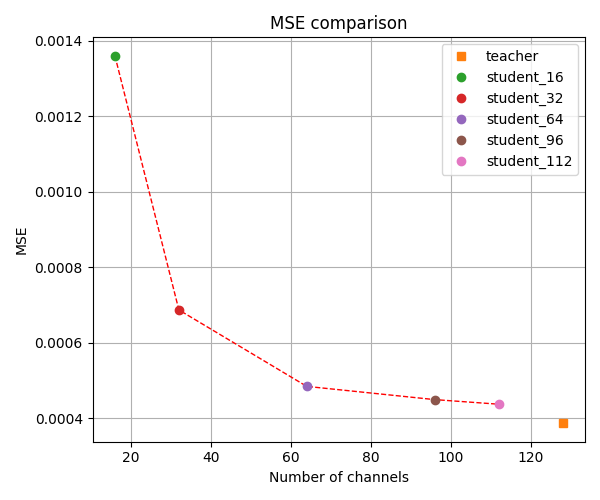
\includegraphics[width=8cm]{../img/kd_ae_mse.png} \label{kd_ae_1:b}}
    \caption[Evaluation on the Kodak dataset of the scale hyperprior student models trained for image reconstruction.]{Evaluation on the Kodak dataset of the scale hyperprior student models trained for image reconstruction. Student models with fewer channels propose less detailed image reconstruction. This is noticeable on single image reconstructions or on average using \acrshort{mse} measures.}
    \label{kd_ae_1}
\end{figure}

For reference, we show in Figure \ref{kd_ae_2} the \acrshort{rd} performance of the student models. It should be noted that the teacher network used in this experiment was trained for image compression tasks so one could argue that these models are not exactly auto-encoders for image reconstruction. What is sure is that they are far from state-of-the-art models in image compression tasks. What remains to be seen is to what extent a properly defined \acrshort{kd} loss for \acrshort{lic} does increase the \acrshort{rd} performance of these student models. This, as well as discussion related to the benefits of smaller student models for \acrshort{lic}, is the subject of the next section.

\begin{figure}
    \centering
    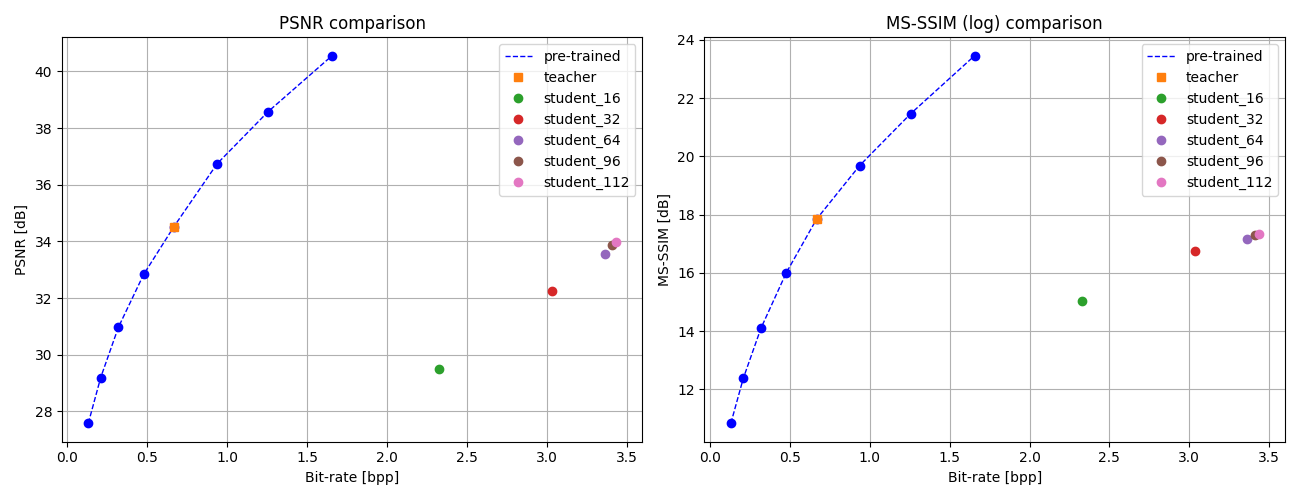
\includegraphics[width=15cm]{../img/kd_ae_rd.png}
    \caption[Average \acrshort{rd} curve on the Kodak dataset for students with different number of channels.]{Average \acrshort{rd} curve on the Kodak dataset for students with different number of channels. Eventhough they were guided by a \acrshort{lic} model during their training, the student models poorly compares to state-of-the-art models in \acrshort{rd}.}
    \label{kd_ae_2}
\end{figure}

Whether it is for custom convolutional \acrshort{ae} or models specifically designed for \acrshort{lic}, there is no denial that \acrshort{kd} positively influence the performance of small models. This section certify this result for image reconstruction, we now transfer this technique to \acrshort{lic} domain.

\section{Knowledge Distillation for Image Compression}
Having assessed the effectiveness of \acrshort{kd} for computer vision tasks similar to image compression, we investigate the success of this frugal \acrshort{ai} technique on \acrshort{nn}-based image compression. Still using the scale hyperprior model introduced in \cite{ballé2018variationalimagecompressionscale}, we train a serie of student models with \acrshort{kd} to evaluate both their \acrshort{rd} performance and their ability to be deployed on resource constrained platforms.

\subsection{Rate-Distortion Performance}
In this section aims at evaluating the \acrshort{rd} performance gain achievable through \acrshort{kd}. By guiding small models during their training with a teacher model, we hope to increase their ability to compress images. We first explain our method then we present our results.

\subsubsection{Method}
\acrshort{lic} distinguish itself from other computer vision tasks (such as dimensionality reduction) by minimising the entropy of the latent representation. In dimensionality reduction, the latent representation has no practical application. When it comes to image compression, it is the latent representation of the image that will be stored or transmitted. Having the smallest possible entropy allows for a smaller entropy coding which means less bits to handle in real world applications. This is why the rate-distortion loss is used in \acrshort{lic} as it allows to find a tradeoff between image quality and bit rate according that fits the requirements of the application. In order to have similar results with \acrshort{lic}, the previous loss function, introduced in Equation \eqref{loss_1}, is updated as follow:

\begin{align}
    L &= \lambda_{1}\, MSE(\hat{y}_{student}, \hat{y}_{teacher}) + \lambda_{2}\, MSE(\hat{x}_{student}, \hat{x}_{teacher}) + \lambda_{3}\, RD(\hat{y}_{student}, \hat{x}_{student}, x)\label{loss_2}
\end{align}

\begin{align}
RD(\hat{y}_{student}, \hat{x}_{student}, x) &= -E[\log_{2}\hat{y}_{student} + \log_{2}\hat{z}_{student}] + \lambda\, MSE(\hat{x}_{student}, x)
\end{align}

\subsubsection{Architecture Size Tradeoff}
\label{architecture_size_tradeoff}
The objective of \acrshort{kd} is to improve the performance of small models using a large one. However, there is no definition of "a small model" so we start by experimenting with model sizes. Following our training method, we create five new models using \acrshort{kd} and the loss function from Equation \ref{loss_2}. We use \(\lambda = 0.025\) in the \acrshort{rd} part of the loss, the same value used by the teacher model during its training. The five models have different sizes. We modify their architecture by changing the number of channels. The smallest deals with as few as 16 channels while the largest student has 112 (number of channels is indicated by the parameter N in Figure \ref{scale_hyperprior_1:b}). It should be noted that the size of the latent space remains the same accross all models, teacher and students.

Unsurprisingly, using \acrshort{RD} loss yields far better results for image compression. Contrary to similar models trained with \acrshort{mse} only (Section \ref{scale_hyperprior_ae}), these new models can be found in the same operational \acrshort{rd} area as state-of-the-art models (Figure \ref{kd_lic_1}).

Results depicted in Figure \ref{kd_lic_1} follow our intuition. Students with larger number of channels (i.e. 64, 96 and 112) take full advantage of \acrshort{kd} and reach roughly the same \acrshort{bpp} and \acrshort{psnr} as the teacher. Models with 16 and 32 channels cannot reach the same level of image quality. Both of them end up far behind pre-trained models in \acrshort{rd} performance and results in higher \acrshort{mse} error (Figure \ref{kd_lic_2:b}). Eventhough they produce visually impressive results (see Figure \ref{kd_lic_2:a}) for models with so few parameters, they are not relevant candidates when taking into account only \acrshort{rd} performance. The number of channels definitely impact the output quality in extreme scenarios (e.g. very few channels) but can be reduced to some extend without degrading image quality.

\begin{figure}
    \centering
    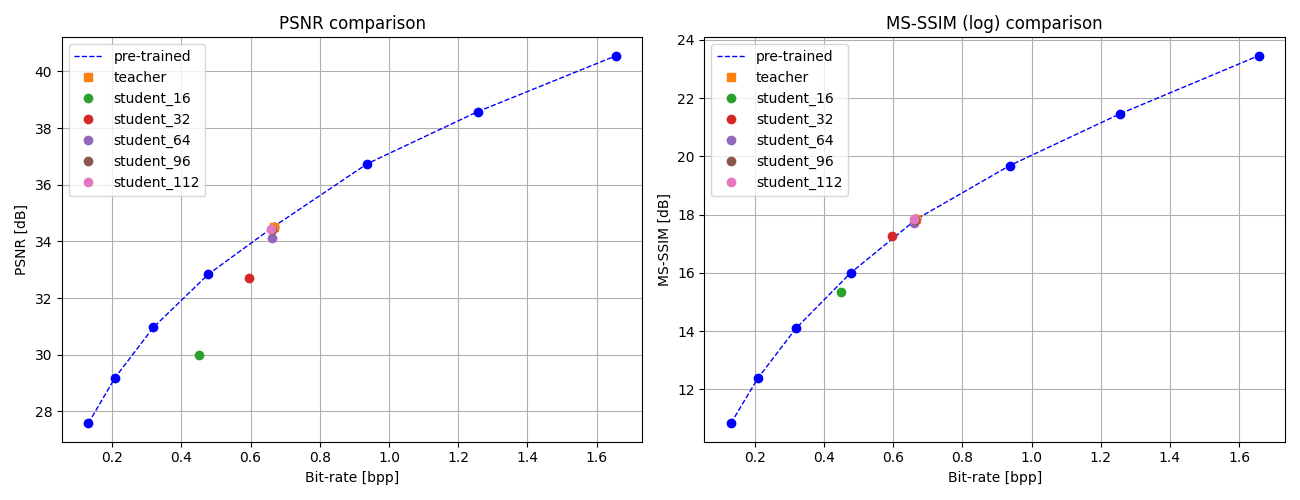
\includegraphics[width=15cm]{../img/kd_lic_rd_channels.png}
    \caption[Average \acrshort{rd} curve on the Kodak dataset for students with different number of channels.]{Average \acrshort{rd} curve on the Kodak dataset for students with different number of channels. Despite being trained similarly, all models have different outputs. Models with at least 64 channels performs alike their teacher but 16 and 32 channels are not sufficient to preserve the same image quality.}
    \label{kd_lic_1}
\end{figure}
% Use 263674, 274457, 274461, 274464, 263691

\begin{figure}[H]
    \centering
    \subfloat[Reconstruction results on image 14 of the Kodak dataset with teacher and student architectures.]{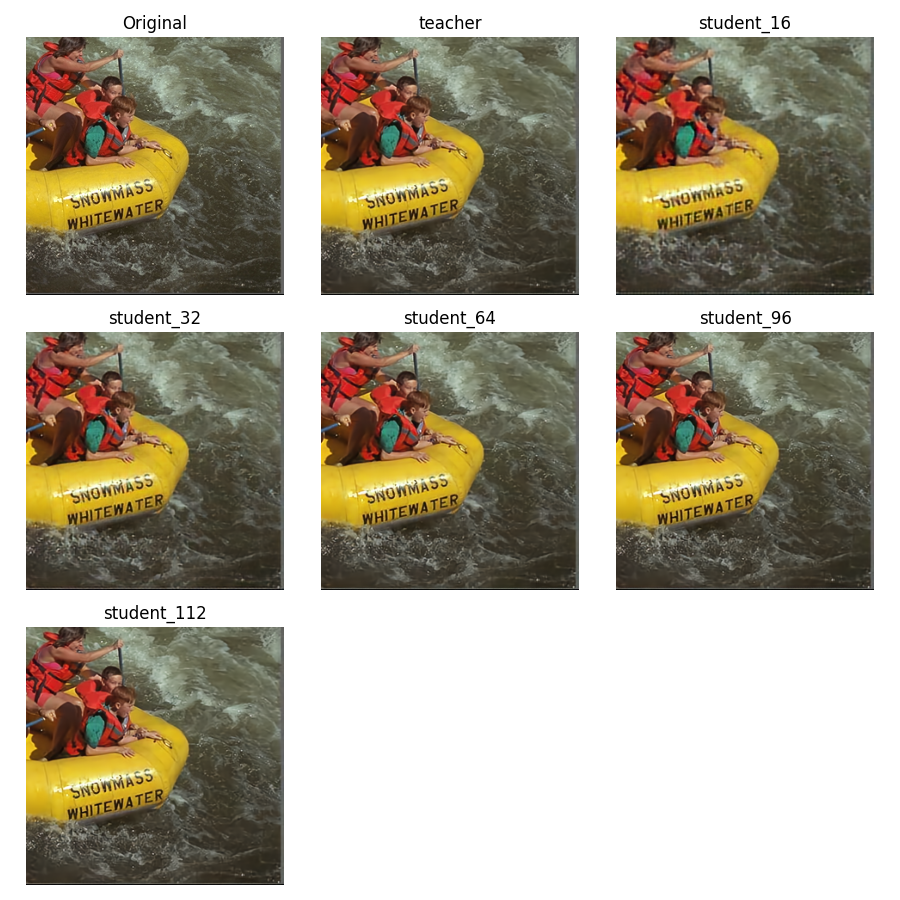
\includegraphics[width=8cm]{../img/kd_lic_kodak_14.png} \label{kd_lic_2:a}}
    \qquad
    \subfloat[Average MSE curve on the Kodak dataset for students with different number of channels.]{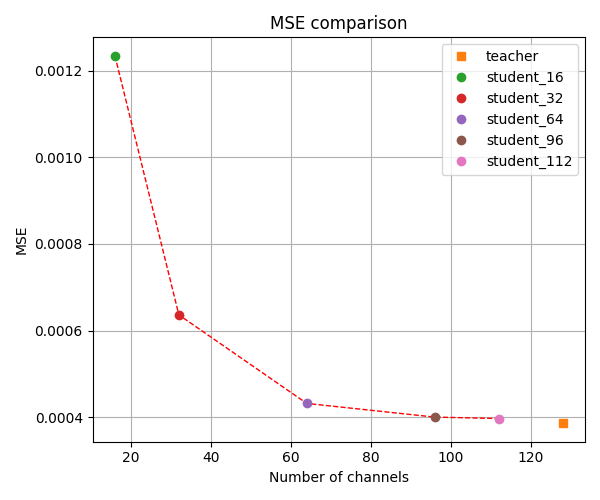
\includegraphics[width=8cm]{../img/kd_lic_mse.png} \label{kd_lic_2:b}}
    \caption[Evaluation on the Kodak dataset of the scale hyperprior student models trained for image compression.]{Evaluation on the Kodak dataset of the scale hyperprior student models trained for image compression. Meticulous visual inspection and average \acrshort{mse} of the output prove the importance of the number of channels when limiting compression loss.}
    \label{kd_lic_2}
\end{figure}

\subsubsection{Rate-Distortion Tradeoff}
Once again, following our training method, we train five new models using \acrshort{kd} and the loss function from Equation \ref{loss_2}. The teacher model is still taken from the compressAI zoo with \textsf{quality} set to 5. This time, we fix the number of channels accross all models (i.e. 64, the smallest number of channels that did not degrade too much performance in previous experiments) but we use different values of \(\lambda\) in the \acrshort{rd} part of the loss. For easier comparison and because our study focuses on low bit rate image compression, we use the values of \(\lambda\) corresponding to the five lowest values of \textsf{quality} (see Table \ref{tab_quality_lambda}). We use the pre-trained models corresponding to the same values of \(\lambda\) as a baseline to compare our results.

As a reminder, the pre-trained models in Figure \ref{kd_lic_4} all have 128 channels. This means that our student models all have half as many channels as the pre-trained models do. Still, all students have similar or higher \acrshort{psnr} than their pre-trained counter-part. More precisely, when quality is prioritised (student 4 and 5), \acrshort{kd} is not the ideal solution: the models performs better than what they would have if trained alone but they are restrained by the modest number of channels. Student 5 attain the limit of what is feasible with 64 channels: with the same \acrshort{rd} tradeoff as the teacher, it is not able to match the teacher image quality. However, smaller models (student 1, 2 and 3) trained to prioritise bit rate reach better \acrshort{psnr} thanks to the teacher model (trained to favorise image quality) pulling them toward the top of the chart. Another interesting experiment is to use a teacher trained to prioritize bit rate. In that case, we observe that all students are pushed toward the bottom left of the chart (Figure \ref{appendix:kd_lic_4_bis}). This compromise could be useful for storage or bandwidth critical operations.

\begin{figure}
    \centering
    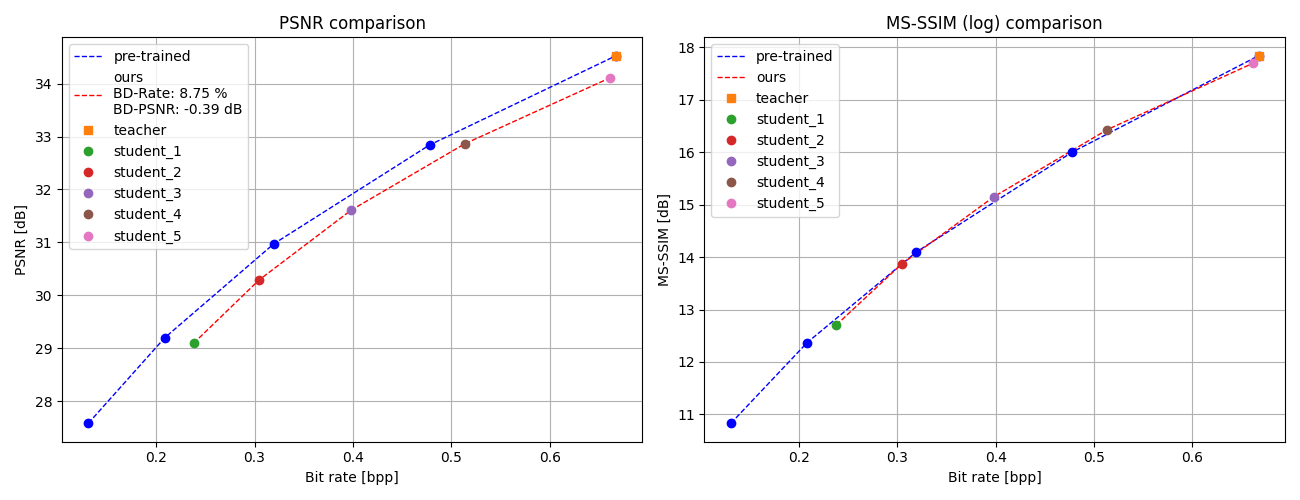
\includegraphics[width=15cm]{../img/kd_lic_rd_lambda_1.png}
    \caption[Average \acrshort{rd} curve on the Kodak dataset for students with different \acrshort{rd} tradeoffs.]{Average \acrshort{rd} curve on the Kodak dataset for students with different \acrshort{rd} tradeoffs. Trained by a teacher with an emphasis on image quality, students 1, 2 and 3 achieve better \acrshort{psnr} than their pre-trained counterpart. Students 4 and 5 are held back by the limited number of channels.}
    \label{kd_lic_4}
\end{figure}
% Use 280392, 281662, 281976, 281979, 274461

This section proves that \acrshort{kd} can be successfully applied to \acrshort{lic} tasks. We are able to train small models with \acrshort{rd} performance almost on par with larger models. But \acrshort{rd} performance is only one part of the equation with frugal \acrshort{ai}: we now need to assess the resource savings. It remains to be seen if it is worth making the tradeoff of loosing some \acrshort{rd} performance to use smaller models.

\subsection{Application to Resource Constrained Platfroms}
\label{application_resource_contrained_platforms}
Real life applications for \acrshort{lic} do not only focus on \acrshort{rd} performance. It is important to ensure great image quality at the lowest bit rate possible but other parameters need to be taken into account. Having proved the effectiveness of \acrshort{kd} for \acrshort{lic} tasks in terms of \acrshort{rd} performance with small student models almost on par with larger models, we now need to put into perspective these results. Let us dive into the second apsect of this study: making \acrshort{lic} possible on resource-limited platforms. This section analyses student models with different architectures from a resource stand point accross three main axis: memory, computing power and energy consumption.

In this section, we use the models first introduced in Section \ref{architecture_size_tradeoff}. There are five student architectures with 16, 32, 64, 96 and 112 channels and a latent space of size 192. We compare our models to pre-trained models from the compressAI zoo (with \textsf{quality} ranging from 1 to 5).

Most resource constrained computers deal with a limited amount of memory. This limiting factor sometimes makes them unsuitable for tasks requiring large models. In \acrshort{lic}, \acrshort{kd} allows to use smaller models without degrading \acrshort{rd} performance. Our student models can have as few as 0.27 M parameters while standard models have 5 M parameters. This is a reduction of up to 95 \% in terms of parameters or memory size. Values for each student model are presented in Table \ref{tab_size}. While the number of parameters definitely impact \acrshort{rd} capabilities of \acrshort{nn}, Figures \ref{kd_lic_parameters} and \ref{appendix:kd_lic_memory} show that student models with 64 channels and above are quite close to their teacher in both \acrshort{psnr} and bit rate. In other words, these model could be used instead of the teacher on devices with limited memory without noticeably degrading the user experience. The student with 64 channels is particularly valuable as it offers \acrshort{psnr} and bit rate inline with the teacher while reducing the memory footprint by 68 \%.

\begin{figure}
    \centering
    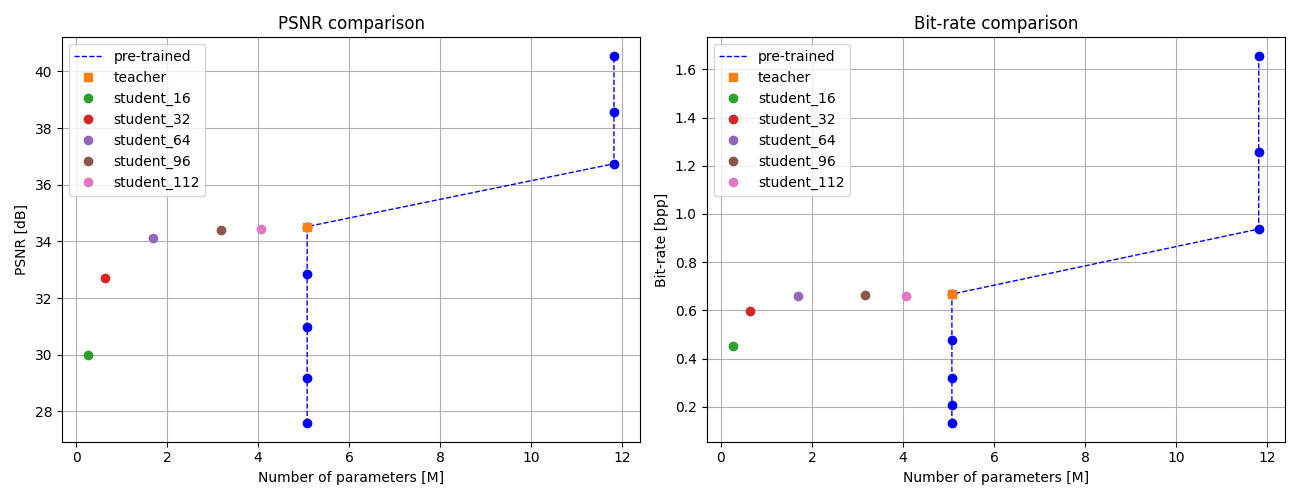
\includegraphics[width=15cm]{../img/kd_lic_parameters.png}
    \caption[\acrshort{psnr} and bit rate on the Kodak dataset according to students number of parameters.]{\acrshort{psnr} and bit rate on the Kodak dataset according to students number of parameters. Reducing the number of parameters graduatly decrease \acrshort{rd} results. Similar results are observed for memory footprint. In our testing, a fair balance between \acrshort{rd} and memory footprint is using 64 channels as it virtually does not degrade performance while reducing the memory footprint by 68 \%.}
    \label{kd_lic_parameters}
\end{figure}

\begin{table}[]
    \centering
    \begin{tabular}{|c|c|lr|lr|lr|lr|}
        \hline
        Model                    & \begin{tabular}[c]{@{}c@{}}Number\\ of channels\end{tabular} & \multicolumn{2}{c|}{\begin{tabular}[c]{@{}c@{}}Number of\\ parameters {[}M{]}\end{tabular}} & \multicolumn{2}{c|}{\begin{tabular}[c]{@{}c@{}}Memory\\ footprint {[}MB{]}\end{tabular}} & \multicolumn{2}{c|}{PSNR} & \multicolumn{2}{c|}{\begin{tabular}[c]{@{}c@{}}Bit rate\\ {[}bpp{]}\end{tabular}} \\ \hline
        Teacher                  & 128                                                          & {\color[HTML]{656565} }                          & 5.08                                     & {\color[HTML]{656565} }                        & 20.18 & {\color[HTML]{656565} }          & 34.53 & {\color[HTML]{656565} }          & 0.67 \\ \hline
        \multirow{5}{*}{Student} & 112                                                          & {\color[HTML]{656565} -19.77 \%}                 & 4.07                                     & {\color[HTML]{656565} -23.03 \%}               & 15.53 & {\color[HTML]{656565} -0.26 \%}  & 34.44 & {\color[HTML]{656565} -1.03 \%}  & 0.66 \\ \cline{2-10} 
                                 & 96                                                           & {\color[HTML]{656565} -37.47 \%}                 & 3.17                                     & {\color[HTML]{656565} -40.01 \%}               & 12.11 & {\color[HTML]{656565} -0.33 \%}  & 34.41 & {\color[HTML]{656565} -0.58 \%}  & 0.66 \\ \cline{2-10} 
                                 & 64                                                           & {\color[HTML]{656565} -66.62 \%}                 & 1.69                                     & {\color[HTML]{656565} -67.98 \%}               & 6.46  & {\color[HTML]{656565} -1.21 \%}  & 34.11 & {\color[HTML]{656565} -0.91 \%}  & 0.66 \\ \cline{2-10}
                                 & 32                                                           & {\color[HTML]{656565} -87.46 \%}                 & 0.64                                     & {\color[HTML]{656565} -87.97 \%}               & 2.43  & {\color[HTML]{656565} -5.25 \%}  & 32.71 & {\color[HTML]{656565} -10.73 \%} & 0.60 \\ \cline{2-10} 
                                 & 16                                                           & {\color[HTML]{656565} -94.77 \%}                 & 0.27                                     & {\color[HTML]{656565} -94.98 \%}               & 1.01  & {\color[HTML]{656565} -13.17 \%} & 29.98 & {\color[HTML]{656565} -32.44 \%} & 0.45 \\ \hline
    \end{tabular}
    \caption[Number of parameters, memory footprint, \acrshort{psnr} and bit rate for teacher and student models.]{Number of parameters, memory footprint, \acrshort{psnr} and bit rate for teacher and student models.}
    \label{tab_size}
\end{table}

Computers can only perform a certain amount of operations per unit of time. When using with mainstream hardware, the computing power required to use an image compression model like the scale hyperprior model is sufficient. However, when dealing with resource constrained devices, the latency might increase which goes against the objective of real-time decompression. With too much latency, it is impossible too extend image decompression to video decompression. Here, we focus on two metrics: the number of \acrfull{flop}s (i.e. the number of floating-point operations carried out to run an inference) and the model throughput (i.e. the number of frames that can process the model in one second). According to our results, the student with 16 channels only requires 3 \% of the teacher \acrshort{flop}s to perform the inference which translates to a 25 \% increase in throughput (see Table \ref{tab_compute}). Figures \ref{kd_lic_flop} and \ref{kd_lic_fps} show that once again, the student with 64 channels represents the best compromise between \acrshort{rd} and \acrshort{flop}s or throughput. It should also be noted that all our models present a throughput that exceeds all requirements for video streaming. This headroom can be used in different ways: we can either increase the stream resolution to enhance user experience or reduce the inference frequency to save energy. 

\begin{figure}
    \centering
    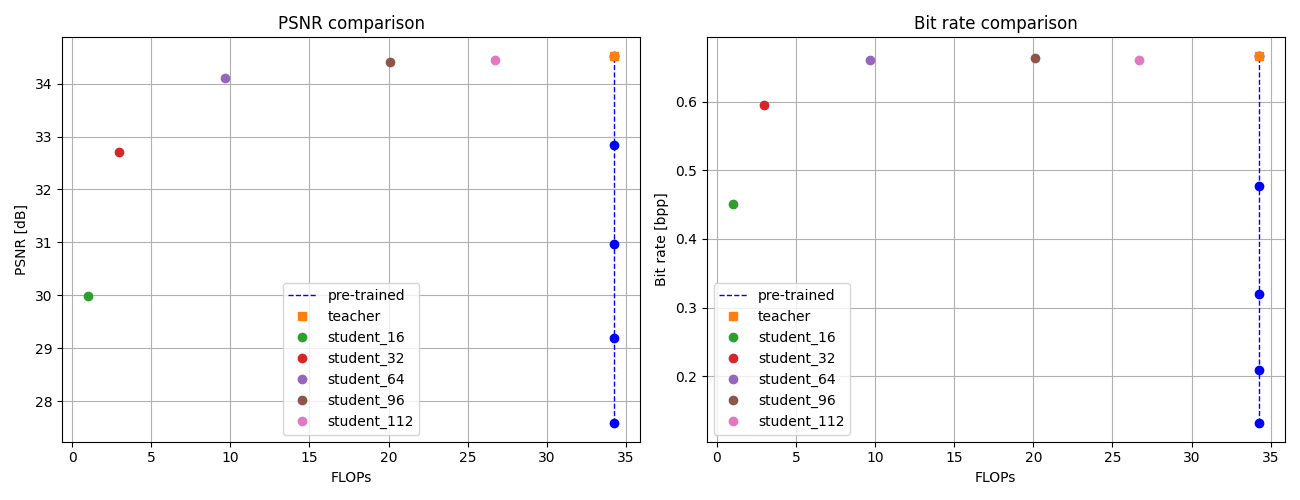
\includegraphics[width=15cm]{../img/kd_lic_flop.png}
    \caption[\acrshort{psnr} and bit rate on the Kodak dataset according to students \acrshort{flop}s.]{\acrshort{psnr} and bit rate on the Kodak dataset according to students \acrshort{flop}s. Our knowledge distilled models are good candidates for devices with limited compute power. They all offer lower \acrshort{flop} counts than standard models. However, this comes at a non-negligeable cost in image quality and bit rate for the smallest models.}
    \label{kd_lic_flop}
\end{figure}

\begin{figure}
    \centering
    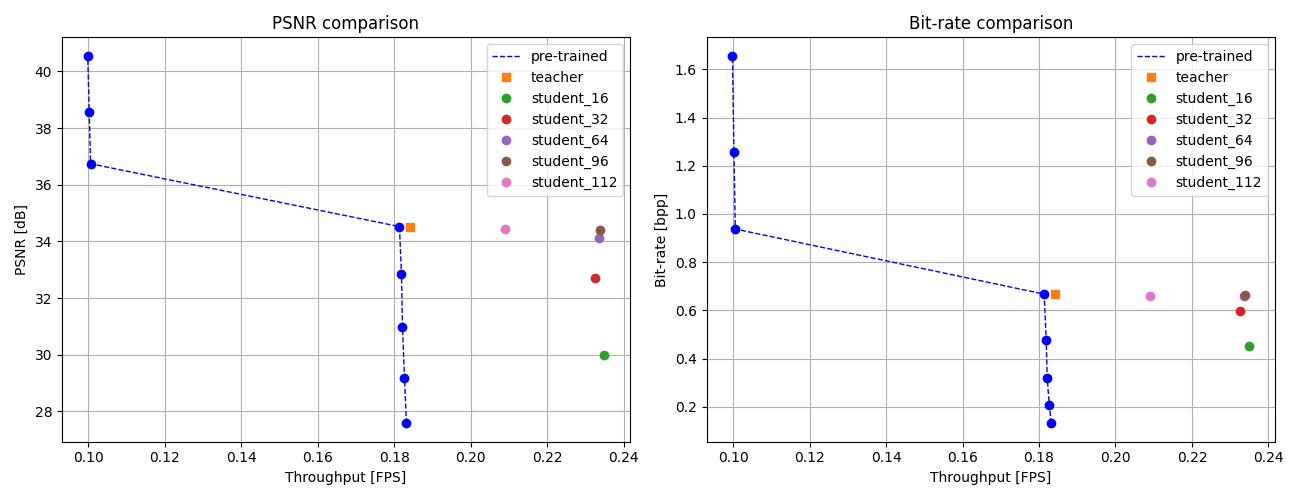
\includegraphics[width=15cm]{../img/kd_lic_fps.png}
    \caption[\acrshort{psnr} and bit rate on the Kodak dataset according to students throughput.]{\acrshort{psnr} and bit rate on the Kodak dataset according to students throughput. All models, exceed standard frame rate. With, higher throughput than pre-trained models, our knowledge distilled models have more headroom for higher resolution frames or lower energy consumption depending the real world application.}
    \label{kd_lic_fps}
\end{figure}

\begin{table}[]
    \centering
    \begin{tabular}{|c|c|lr|lr|lr|lr|}
    \hline
    Model                    & \begin{tabular}[c]{@{}c@{}}Number\\ of channels\end{tabular} & \multicolumn{2}{c|}{\begin{tabular}[c]{@{}c@{}}Floating point\\ operations\\ {[}GFLOP/frame{]}\end{tabular}} & \multicolumn{2}{c|}{\begin{tabular}[c]{@{}c@{}}Throughput\\ {[}FPS{]}\end{tabular}} & \multicolumn{2}{c|}{PSNR} & \multicolumn{2}{c|}{\begin{tabular}[c]{@{}c@{}}Bit rate\\ {[}bpp{]}\end{tabular}} \\ \hline
    Teacher                  & 128                                                          & {\color[HTML]{656565} }                                & 34.24                                             & {\color[HTML]{656565} }                     & 184.20 & {\color[HTML]{656565} }          & 34.53 & {\color[HTML]{656565} }          & 0.67 \\ \hline
    \multirow{5}{*}{Student} & 112                                                          & {\color[HTML]{656565} -22.01 \%}                       & 26.70                                             & {\color[HTML]{656565} +13.47 \%}            & 209.01 & {\color[HTML]{656565} -0.26 \%}  & 34.44 & {\color[HTML]{656565} -1.03 \%}  & 0.66 \\ \cline{2-10} 
                             & 96                                                           & {\color[HTML]{656565} -41.31 \%}                       & 20.10                                             & {\color[HTML]{656565} +25.74 \%}            & 231.61 & {\color[HTML]{656565} -0.33 \%}  & 34.41 & {\color[HTML]{656565} -0.58 \%}  & 0.66 \\ \cline{2-10}
                             & 64                                                           & {\color[HTML]{656565} -71.75 \%}                       & 9.67                                              & {\color[HTML]{656565} +26.20 \%}            & 232.47 & {\color[HTML]{656565} -1.21 \%}  & 34.11 & {\color[HTML]{656565} -0.91 \%}  & 0.66 \\ \cline{2-10} 
                             & 32                                                           & {\color[HTML]{656565} -91.31 \%}                       & 2.98                                              & {\color[HTML]{656565} +25.89 \%}            & 231.90 & {\color[HTML]{656565} -5.25 \%}  & 32.71 & {\color[HTML]{656565} -10.73 \%} & 0.60 \\ \cline{2-10}
                             & 16                                                           & {\color[HTML]{656565} -97.01 \%}                       & 1.02                                              & {\color[HTML]{656565} +26.83 \%}            & 233.63 & {\color[HTML]{656565} -13.17 \%} & 29.98 & {\color[HTML]{656565} -32.44 \%} & 0.45 \\ \hline
    \end{tabular}
    \caption[\acrshort{flop}s, throughput, \acrshort{psnr} and bit rate for teacher and student models.]{\acrshort{flop}s, throughput, \acrshort{psnr} and bit rate for teacher and student models.}
    \label{tab_compute}
\end{table}

Most edge devices also have access to a limited amount of energy whether it is in time because they run on battery like smartphones or because they are \acrfull{iot} devices that run 24/7 and thus should not consume a lot of energy. This is why we focus on the energy required to process a single frame. Table \ref{tab_energy} shows that we can save up to 60 \% of the energy used by the teacher model by using the student with 16 channels. Using Figure \ref{kd_lic_energy}, that the model that offers the best tradeoff between \acrshort{psnr} and energy consumption in the student model with 64 channels. By using this model we keep the same image quality while reducing our energy consumption by 35 \%.

\begin{figure}
    \centering
    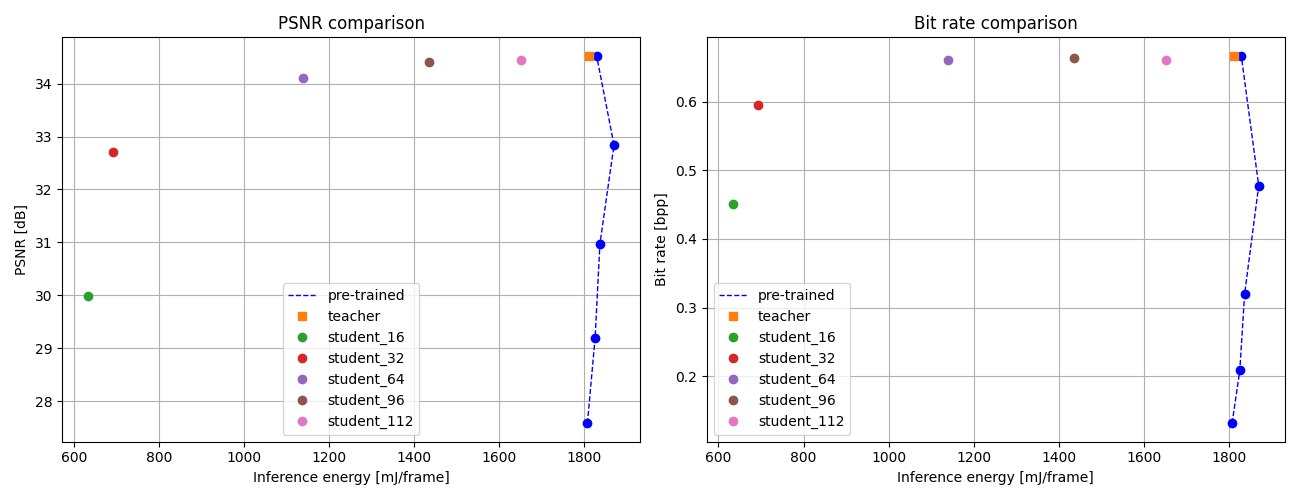
\includegraphics[width=15cm]{../img/kd_lic_energy.png}
    \caption[\acrshort{psnr} and bit rate on the Kodak dataset according to students consumed energy.]{\acrshort{psnr} and bit rate on the Kodak dataset according to students consumed energy. \acrshort{kd} is a great method to create energy friendly \acrshort{lic} models. If energy consumption is not too restricted, we recommand using the student with 64 channels that consumes 35 \% less energy per frame and achieve image compression on par with the teacher model.}
    \label{kd_lic_energy}
\end{figure}

\begin{table}[]
    \centering
    \begin{tabular}{|c|c|lr|lr|lr|}
        \hline
        Model                    & \begin{tabular}[c]{@{}c@{}}Number\\ of channels\end{tabular} & \multicolumn{2}{c|}{\begin{tabular}[c]{@{}c@{}}Energy\\ {[}mJ/frame{]}\end{tabular}} & \multicolumn{2}{c|}{PSNR} & \multicolumn{2}{c|}{\begin{tabular}[c]{@{}c@{}}Bit rate\\ {[}bpp{]}\end{tabular}} \\ \hline
        Teacher                  & 128                                                          & {\color[HTML]{656565} }                     & 1767.85 & {\color[HTML]{656565} }          & 34.53 & {\color[HTML]{656565} }          & 0.67 \\ \hline
        \multirow{5}{*}{Student} & 112                                                          & {\color[HTML]{656565} -9.47 \%}             & 1600.41 & {\color[HTML]{656565} -0.26 \%}  & 34.44 & {\color[HTML]{656565} -1.03 \%}  & 0.66 \\ \cline{2-8} 
                                 & 96                                                           & {\color[HTML]{656565} -19.88 \%}            & 1416.34 & {\color[HTML]{656565} -0.33 \%}  & 34.41 & {\color[HTML]{656565} -0.58 \%}  & 0.66 \\ \cline{2-8}
                                 & 64                                                           & {\color[HTML]{656565} -34.15 \%}            & 1164.17 & {\color[HTML]{656565} -1.21 \%}  & 34.11 & {\color[HTML]{656565} -0.91 \%}  & 0.66 \\ \cline{2-8}
                                 & 32                                                           & {\color[HTML]{656565} -60.45 \%}            & 699.18  & {\color[HTML]{656565} -5.25 \%}  & 32.71 & {\color[HTML]{656565} -10.73 \%} & 0.60 \\ \cline{2-8}
                                 & 16                                                           & {\color[HTML]{656565} -61.28 \%}            & 684.45  & {\color[HTML]{656565} -13.17 \%} & 29.98 & {\color[HTML]{656565} -32.44 \%} & 0.45 \\ \hline
    \end{tabular}
    \caption[Consumed energy, \acrshort{psnr} and bit rate for teacher and student models.]{Consumed energy, \acrshort{psnr} and bit rate for teacher and student models.}
    \label{tab_energy}
\end{table}

This section is a deep dive into the resource consumption of standard and knowledge distilled models. Based on measures of memory usage, required computing power and energy consumption on students architectures with varying number of channels, we prove that \acrshort{kd} indeed create frugal models. In all experiments, our \acrshort{kd} models consume less resources that standard models at a (sometimes negligeable) cost in \acrshort{rd} performance. On a not-too-constrained platform, we would recommand the use of the student with 64 channels. It has a limited use of resources without noticeable impact on image compression.

This chapter is a step in the right direction for \acrshort{lic} on resource constrained platforms. We first assess the effectiveness of \acrshort{kd} on well known models and tasks then transfer this frugal \acrshort{ai} technique to \acrshort{lic}. \acrshort{rd} results are impressive, showing models with as low as half as many channels in the same operational region as their teacher. We also experiment with different teachers and find that we can train student models adapted for any image compression/resource consumption tradeoff possible. Other settings like the loss function definitely impact the student performances, leaving room for other research work. Most importantly, we measure a significant reduction in the model resource consumption (memory, compute, and energy) without too much degradation of the image compression \acrhsort{rd}. We observe that \acrshort{kd} is a valuable training paradigm in order to achieve real-time image compression on resource limited devices.

\chapter*{Conclusion}
\addcontentsline{toc}{chapter}{Conclusion}
Data compression and especially image compression is a crucial tool in information technology. Whether it is to save storage space or to improve networks efficiency, the goal is to represent the same information with the minimum amount of bits. Lossless compression is limited, leaving place to lossy compression. This compression method introduces a tradeoff between storage space and data quality/integrity.

Using existing deep learning and computer vision tools, \acrfull{lic} aims to provide a new way to perform image compression providing better results than previous deterministic codecs. \acrshort{lic} requires a lot of processing power making it unsusable on resource constrained platforms.

The final goal of this project is to explore technique allowing to use \acrshort{lic} on these low power devices possibly in real-time. After reproducing state of the art results, the goal is to explore frugal machine learning techniques such as pruning, quantisation and knowledge distillation.

\printbibliography

\appendix

\chapter{Reproducibility}

\section{Implementation Details}
Here is a list of useful details regarding our implementation:
\begin{itemize}
    \item Python 3.12.7
    \item Anaconda virtual environment
    \item compressAI 1.2.6
    \item Code hosted on private GitHub repository
    \item Processing power provided by Télécom Paris GPU cluster (\url{https://docs.google.com/document/d/1lXykfpEUJCrbNh22D2f2kxNS0gV6t-j9A_juWFdiEnI/edit?tab=t.0})
\end{itemize}

\section{Measures}

% TODO

\chapter{Figures}

\begin{figure}
    \centering
    \includegraphics[width=15cm]{img/kd_ae_kodak_14.png}
    \caption[Evaluation on the Kodak dataset of the scale hyperprior student models trained for image compression: reconstruction results on image 14 of the Kodak dataset with teacher and student architectures.]{Evaluation on the Kodak dataset of the scale hyperprior student models trained for image compression: reconstruction results on image 14 of the Kodak dataset with teacher and student architectures.}
    \label{appendix:kd_ae_1}
\end{figure}

\begin{figure}
    \centering
    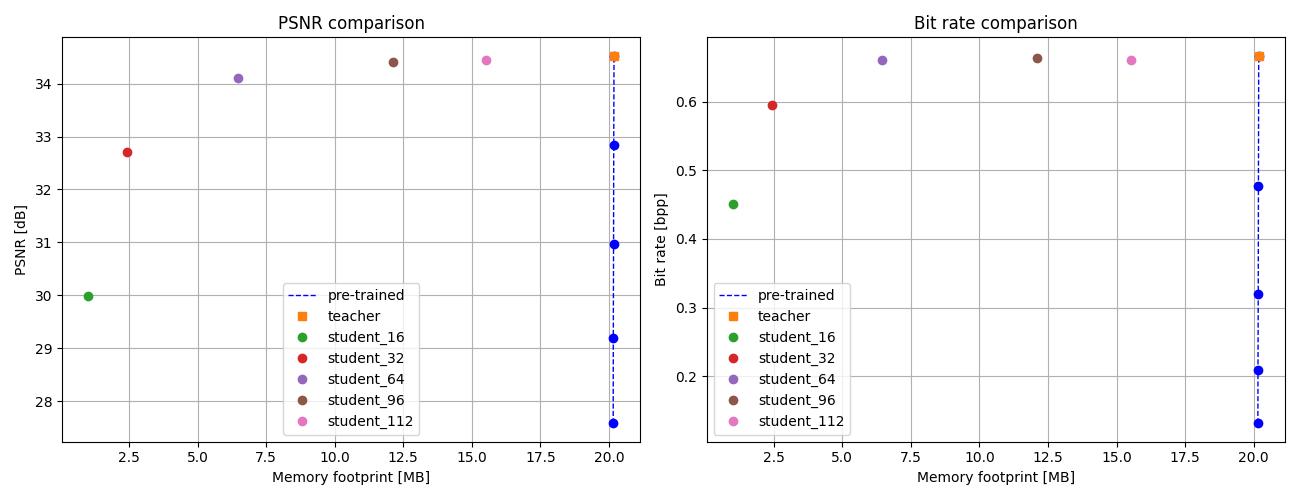
\includegraphics[width=15cm]{img/kd_lic_memory.png}
    \caption[\acrshort{psnr} and bit rate on the Kodak dataset according to students memory footprint.]{\acrshort{psnr} and bit rate on the Kodak dataset according to students memory footprint.}
    \label{appendix:kd_lic_memory}
\end{figure}

\begin{figure}
    \centering
    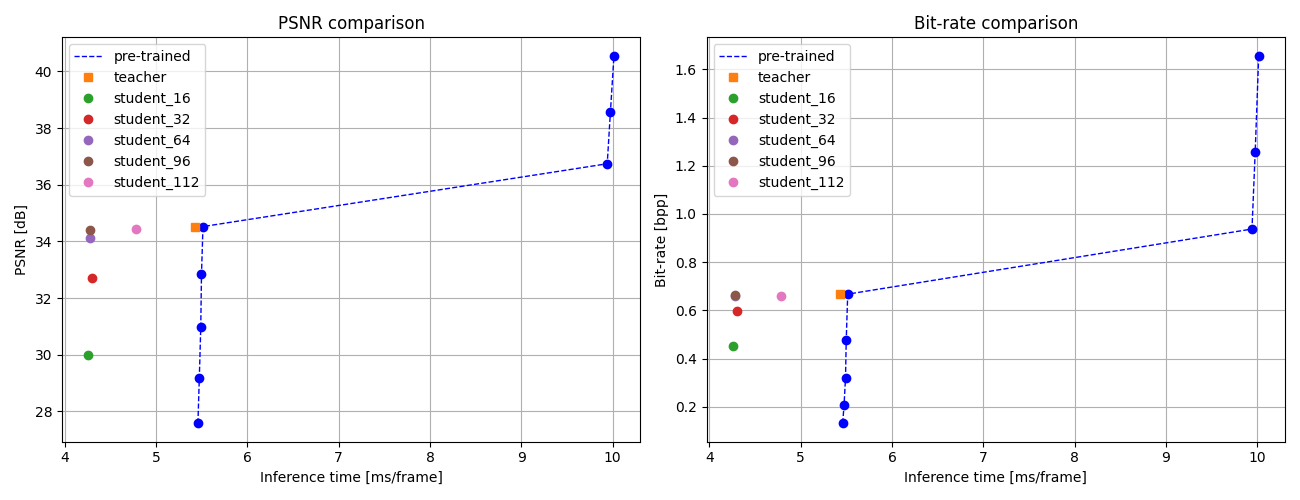
\includegraphics[width=15cm]{img/kd_lic_time.png}
    \caption[\acrshort{psnr} and bit rate on the Kodak dataset according to students inference time.]{\acrshort{psnr} and bit rate on the Kodak dataset according to students inference time.}
    \label{appendix:kd_lic_time}
\end{figure}

\begin{sidewaystable}[]
    \centering
    \begin{tabular}{|c|c|lr|lr|lr|lr|lr|lr|lr|}
        \hline
        Model                     & \begin{tabular}[c]{@{}c@{}}Number\\ of channels\end{tabular} & \multicolumn{2}{c|}{\begin{tabular}[c]{@{}c@{}}Number of\\ parameters {[}M{]}\end{tabular}} & \multicolumn{2}{c|}{\begin{tabular}[c]{@{}c@{}}Memory\\ footprint {[}MB{]}\end{tabular}} & \multicolumn{2}{c|}{\begin{tabular}[c]{@{}c@{}}Floating point\\ operations\\ {[}GFLOP/frame{]}\end{tabular}} & \multicolumn{2}{c|}{\begin{tabular}[c]{@{}c@{}}Throughput\\ {[}FPS{]}\end{tabular}} & \multicolumn{2}{c|}{\begin{tabular}[c]{@{}c@{}}Energy\\ {[}mJ/frame{]}\end{tabular}} & \multicolumn{2}{c|}{PSNR}               & \multicolumn{2}{c|}{\begin{tabular}[c]{@{}c@{}}Bit rate\\ {[}bpp{]}\end{tabular}}      \\ \hline
        Teacher                   & 128                        & {\color[HTML]{656565} }                                  & 5.08                         & {\color[HTML]{656565} }                                  & 20.18                        & {\color[HTML]{656565} }                                  & 34.24                        & {\color[HTML]{656565} }                                  & 184.20                         & {\color[HTML]{656565} }                                  & 1767.85                         & {\color[HTML]{656565} }                                 & 34.53                         & {\color[HTML]{656565} }                                 & 0.67                         \\ \hline
                                  & 112                        & {\color[HTML]{656565} -19.77 \%}                         & 4.07                         & {\color[HTML]{656565} -23.03 \%}                         & 15.53                        & {\color[HTML]{656565} -22.01 \%}                         & 26.70                        & {\color[HTML]{656565} +13.47 \%}                         & 209.01                         & {\color[HTML]{656565} -9.47 \%}                          & 1600.41                         & {\color[HTML]{656565} -0.26 \%}                         & 34.44                         & {\color[HTML]{656565} -1.03 \%}                         & 0.66                         \\ \cline{2-16} 
                                  & 96                         & {\color[HTML]{656565} -37.47 \%}                         & 3.17                         & {\color[HTML]{656565} -40.01 \%}                         & 12.11                        & {\color[HTML]{656565} -41.31 \%}                         & 20.10                        & {\color[HTML]{656565} +25.74 \%}                         & 231.61                         & {\color[HTML]{656565} -19.88 \%}                         & 1416.34                         & {\color[HTML]{656565} -0.33 \%}                         & 34.41                         & {\color[HTML]{656565} -0.58 \%}                         & 0.66                         \\ \cline{2-16} 
                                  & \cellcolor[HTML]{EFEFEF}64 & \cellcolor[HTML]{EFEFEF}{\color[HTML]{656565} -66.62 \%} & \cellcolor[HTML]{EFEFEF}1.69 & \cellcolor[HTML]{EFEFEF}{\color[HTML]{656565} -67.98 \%} & \cellcolor[HTML]{EFEFEF}6.46 & \cellcolor[HTML]{EFEFEF}{\color[HTML]{656565} -71.75 \%} & \cellcolor[HTML]{EFEFEF}9.67 & \cellcolor[HTML]{EFEFEF}{\color[HTML]{656565} +26.20 \%} & \cellcolor[HTML]{EFEFEF}232.47 & \cellcolor[HTML]{EFEFEF}{\color[HTML]{656565} -34.15 \%} & \cellcolor[HTML]{EFEFEF}1164.17 & \cellcolor[HTML]{EFEFEF}{\color[HTML]{656565} -1.21 \%} & \cellcolor[HTML]{EFEFEF}34.11 & \cellcolor[HTML]{EFEFEF}{\color[HTML]{656565} -0.91 \%} & \cellcolor[HTML]{EFEFEF}0.66 \\ \cline{2-16} 
                                  & 32                         & {\color[HTML]{656565} -87.46 \%}                         & 0.64                         & {\color[HTML]{656565} -87.97 \%}                         & 2.43                         & {\color[HTML]{656565} -91.31 \%}                         & 2.98                         & {\color[HTML]{656565} +25.89 \%}                         & 231.90                         & {\color[HTML]{656565} -60.45 \%}                         & 699.18                          & {\color[HTML]{656565} -5.25 \%}                         & 32.71                         & {\color[HTML]{656565} -10.73 \%}                        & 0.60                         \\ \cline{2-16} 
        \multirow{-5}{*}{Student} & 16                         & {\color[HTML]{656565} -94.77 \%}                         & 0.27                         & {\color[HTML]{656565} -94.98 \%}                         & 1.01                         & {\color[HTML]{656565} -97.01 \%}                         & 1.02                         & {\color[HTML]{656565} +26.83 \%}                         & 233.63                         & {\color[HTML]{656565} -61.28 \%}                         & 684.45                          & {\color[HTML]{656565} -13.17 \%}                        & 29.98                         & {\color[HTML]{656565} -32.44 \%}                        & 0.45                         \\ \hline
    \end{tabular}
    \caption{}
    \label{appendix:tab_resources}
\end{sidewaystable}

% \vspace*{-2cm}
% \chapter*{Abstract}
\addcontentsline{toc}{chapter}{Abstract}


\end{document}